% Author: Victor Terron (c) 2013
% Email: `echo vt2rron1iaa32s | tr 132 @.e`
% License: GNU GPLv3

\documentclass[14pt]{beamer}

\usepackage[utf8]{inputenc}

\usetheme{Copenhagen}
\useoutertheme{infolines}
\setbeamercovered{dynamic}

\title{Cuarenta características de Python\\ que quizás no conoces}
\author{Víctor Terrón}
\date{23 de noviembre de 2013}
\institute{IAA-CSIC}

\begin{document}

\begin{frame}
  \titlepage
  \begin{figure}
    \vspace{-0.5cm}
    
\includegraphics[width=3cm]{pics/mistery-box.jpg}
  \end{figure}
\end{frame}

\section{Introducción}

\begin{frame}{Unknown Unknowns}
  \small
  \begin{block}{}
    \centering
    ``There are things we know that we know. There are known
    unknowns. That is to say there are things that we now know we
    don't know. But there are also \structure{unknown unknowns}. There
    are things we do not know we don't know'' [Donald Rumsfeld, 2002]
  \end{block}

  \small
  \begin{itemize}
    \item En Python hay funcionalidades increíbles,
     \structure{imprescindibles una vez que las conoces}, que
     podríamos no echar en falta jamás porque ni siquiera sabíamos
     que existían.
    \item El propósito de esta charla es presentar una serie de
      aspectos interesantes de Python que en estos años he descubierto
      que mucha gente, incluso programadores veteranos, desconoce.
  \end{itemize}
\end{frame}

\begin{frame}{Unknown Unknowns}
  \begin{itemize}
    \item Algunas de las funcionalidades que vamos a discutir aquí son
      muy prácticas y otras curiosidades de indiscutiblemente escasa o
      nula utilidad en nuestro día a día. Pero todos ellos son
      conceptos \structure{sencillos de entender} y que merece la pena
      saber que están ahí, incluso si no los usamos... por ahora.
    \item Tenemos 1:15 minutos para cada uno de los puntos, así que
      muchos de ellos sólo vamos a poder \structure{verlos muy por
      encima}. Pero al menos habrán dejado de ser \emph{unknown
      unknowns}.
  \end{itemize}
\end{frame}

\begin{frame}{¡No os limitéis a escuchar!}
  \begin{center}
    No suele ser divertido escuchar a nadie hablar durante casi una
    hora. Participad, intervenid, criticad, opinad. ¡Si digo algo que
    no tiene ningún sentido, \structure{corregidme}!
  \end{center}

  \begin{block}{\centering El código fuente está disponible en:}
    \centering \url{http://github.com/vterron/PyConES-2013}
  \end{block}

  \begin{center}
    \small Erratas, correcciones, enlaces interesantes...\\ ¿enviará
    alguien algún pull request antes de que termine esta charla?
  \end{center}
\end{frame}

\begin{frame}{}
  \begin{alertblock}{}
    \centering \Large ¿Listos?
  \end{alertblock}

  \begin{figure}
    \centering
    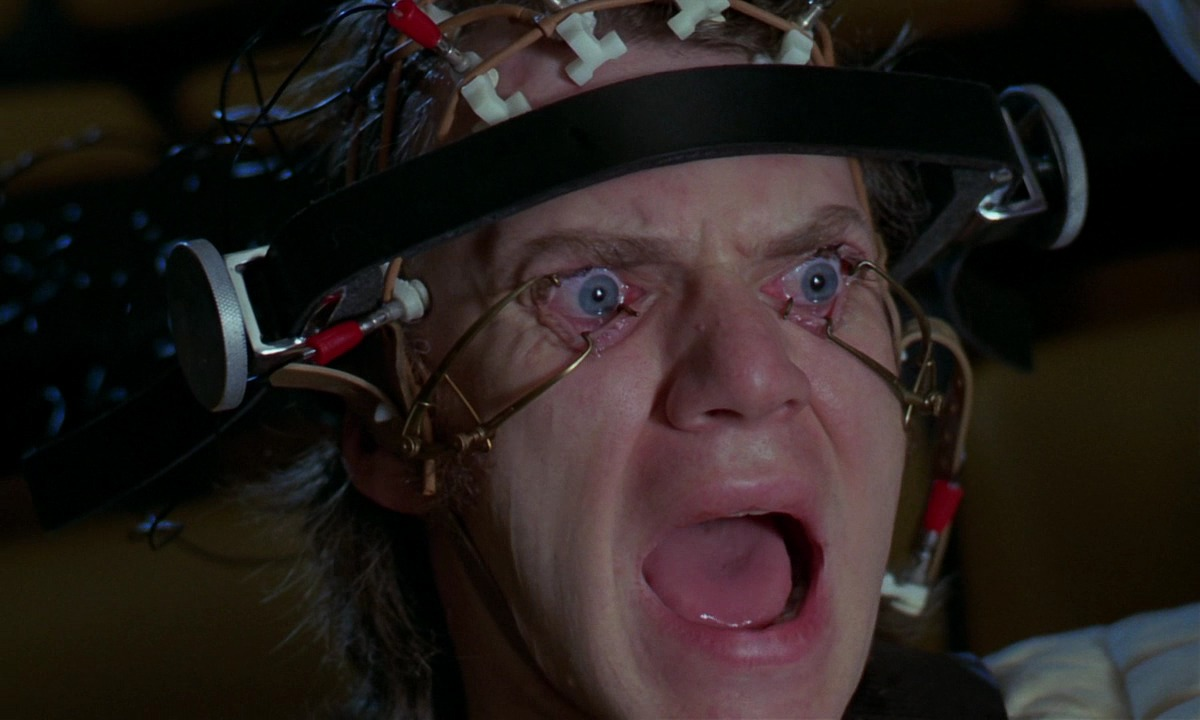
\includegraphics[height=6cm]{pics/a-clockwork-orange.jpg}
  \end{figure}
\end{frame}

\end{document}

